\definecolor{red1}{RGB}{228,26,28}
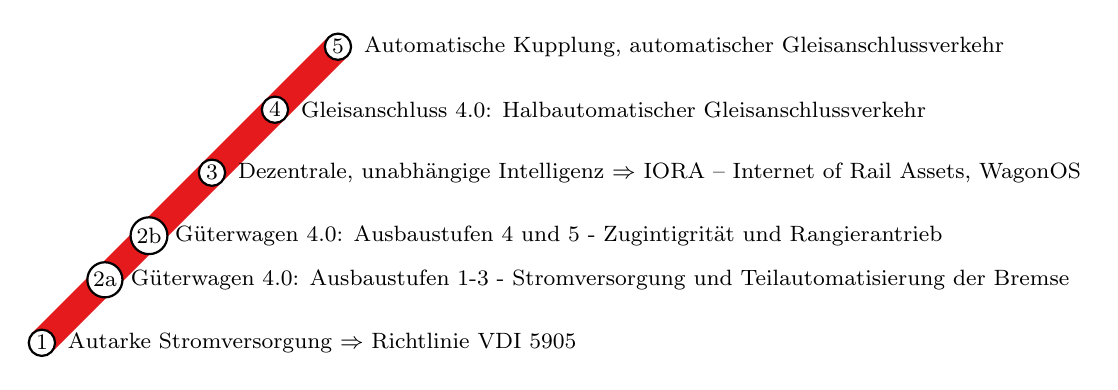
\begin{tikzpicture}[font = \sffamily, scale = 0.8]
\tikzstyle{every node}=[font=\footnotesize]
\path[line width = .35cm, draw = red1] (0,0) -- (4.7,4.7);
\path[draw, thick, fill = white] (0,0) node[circle, draw, fill = white, inner sep = 1] {1}  node[xshift = .2cm, anchor = west] {Autarke Stromversorgung $\Rightarrow$ Richtlinie VDI 5905};

\path[draw, thick, fill = white] (1,1) node[circle, draw, fill = white, inner sep = 1] {2a} node[xshift = .2cm, anchor = west] {Güterwagen 4.0: Ausbaustufen 1-3 - Stromversorgung und Teilautomatisierung der Bremse};
\path[draw, thick, fill = white] (1.7,1.7) node[circle, draw, fill = white, inner sep = 1] {2b}  node[xshift = .2cm, anchor = west] {Güterwagen 4.0: Ausbaustufen 4 und 5 - Zugintigrität und  Rangierantrieb};

\path[draw, thick, fill = white] (2.7,2.7) node[circle, draw, fill = white, inner sep = 1] {3}  node[xshift = .2cm, anchor = west] {Dezentrale, unabhängige Intelligenz $\Rightarrow$ IORA -- Internet of Rail Assets, WagonOS};
\path[draw, thick, fill = white] (3.7,3.7) node[circle, draw, fill = white, inner sep = 1] {4}  node[xshift = .2cm, anchor = west] {Gleisanschluss 4.0: Halbautomatischer Gleisanschlussverkehr};
\path[draw, thick, fill = white] (4.7,4.7) node[circle, draw, fill = white, inner sep = 1] {5}  node[xshift = .2cm, anchor = west] {Automatische Kupplung, automatischer Gleisanschlussverkehr};
\end{tikzpicture}